\documentclass{beamer}

\mode<presentation>
{
\usetheme{Frankfurt}

\setbeamercovered{transparent}
}

\usepackage[russian]{babel}
\usepackage[utf8]{inputenc}


\usepackage{mathptmx}
\usepackage{graphics}
\usepackage[scaled=.90]{helvet}
\usepackage{courier}

\usepackage[T1]{fontenc}


\title{Парадигмы программрования мобильных роботов на примере системы АМУР}

%\subtitle{}

% - Use the \inst{?} command only if the authors have different
%   affiliation.
%\author{F.~Author\inst{1} \and S.~Another\inst{2}}
\author{Кирсанов К.Б.}

% - Use the \inst command only if there are several affiliations.
% - Keep it simple, no one is interested in your street address.

\institute[sensorika]
{Международная Лаборатория Сенсорика}

\date{07.06.12 / XIII Международный образовательный форум
«Интеллектуальное пространство»}

% If you have a file called "university-logo-filename.xxx", where xxx
% is a graphic format that can be processed by latex or pdflatex,
% resp., then you can add a logo as follows:

% \pgfdeclareimage[height=0.5cm]{university-logo}{university-logo-filename}
% \logo{\pgfuseimage{university-logo}}

% If you wish to uncover everything in a step-wise fashion, uncomment
% the following command:

%\beamerdefaultoverlayspecification{<+->}

\begin{document}

\begin{frame}
\titlepage
\end{frame}

\begin{frame}
\frametitle{Содержание}
\tableofcontents
\end{frame}

\section{Роботы в образовательной среде}
\subsection{Роботы как учебные пособия и объекты лабораторных работ}
\begin{frame}
\frametitle{Роботы как учебные пособия и объекты лабораторных работ}
Использование мобильных роботов в качестве учебных объектов повышает
заинтересованность учащихся
\\
\begin{itemize}
  \item<1> Решение реальных, а не учебных задач: навигация, обеспечение
  взаимодействия с человеком, синтез речи, алгоритмы поиска, механика.
  \item<1> Интерактивность, не доступная в моделях - любая ошибка становиться тут
  же заметной
  \item<1> Широта охватываемых задач, - от программирования и механики, до
  лингвистики и дизайна
\end{itemize}
\end{frame}

\section{Программирование мобильных роботов}
\subsection{Существующие общедоступные системы}
\begin{frame}
\frametitle{Системы программирования}
\begin{itemize}
\item<1> \textbf{Robotino View} \textit{http://wiki.openrobotino.org/}
\item<1> \textbf{Microsoft Robotics Studio}
\textit{http://msdn.microsoft.com/en-us/robotics/default.aspx}
\item<1> \textbf{Player Project} \textit{http://playerstage.sourceforge.net}
\item<1> \textbf{ORCA2} \textit{http://orca-robotics.sourceforge.net/orca/index.html}
\item<1> \textbf{LAAS/GenoM} \textit{https://softs.laas.fr/openrobots/wiki/genom}
\item<1> \textbf{Marie} \textit{http://marie.sourceforge.net}
\item<1> \textbf{URBI} \textit{http://www.urbiforge.com}
\item<1> \textbf{Webots} \textit{http://www.cyberbotics.com}
\item<1> \textbf{RoboJRE} \textit{http://www.ridgesoft.com/robojde/robojde.htm}
\item<1> \textbf{OROCOS} \textit{http://www.orocos.org}
\item<1> \textbf{LEGO, iRobot, ...}
\end{itemize}
\end{frame}

%\subsection{Ключевые абстракции}
\subsection{Языки программирования}
\begin{frame}
\frametitle{Языки программирования}
Как правило используются распространенные императивные языки: C/C++, Java, C#,
matlab, python.
\\
Для этих языков выпускаются библиотеки функций и классов, абстрагирующие работу
с роботом.
\\
\\
 
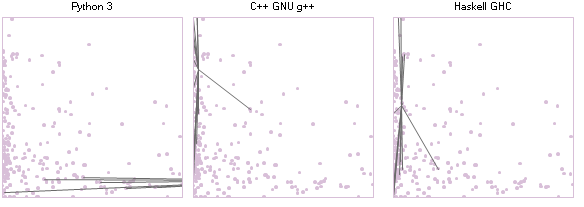
\includegraphics[scale=0.5]{languages.png}
\\
размер кода/производительность для различных языков

\end{frame}

\subsection{Проблемно-ориентированные языки}
\begin{frame}
\frametitle{Проблемно-ориентированные языки}
Предметно-ориентированный язык программирования (domain-specific language, DSL)
-- язык программирования, специально разработанный для решения определённого
круга задач.

\\

``Старые'' языки (С/С++, matlab) почти не расширяемы, в то время как ``новые''
(Python, C#, Java) могут служить основой новых языков. Наиболее удобны для
реализации DSL мало-популярные языки, - Haskell, Scala(Lisp), Clean и т.п.

\end{frame}


\subsubsection{Визуальные(графовые) языки}
\begin{frame}
\frametitle{Визуальные(графовые) языки}
\framesubtitle{Показывается в реламе}
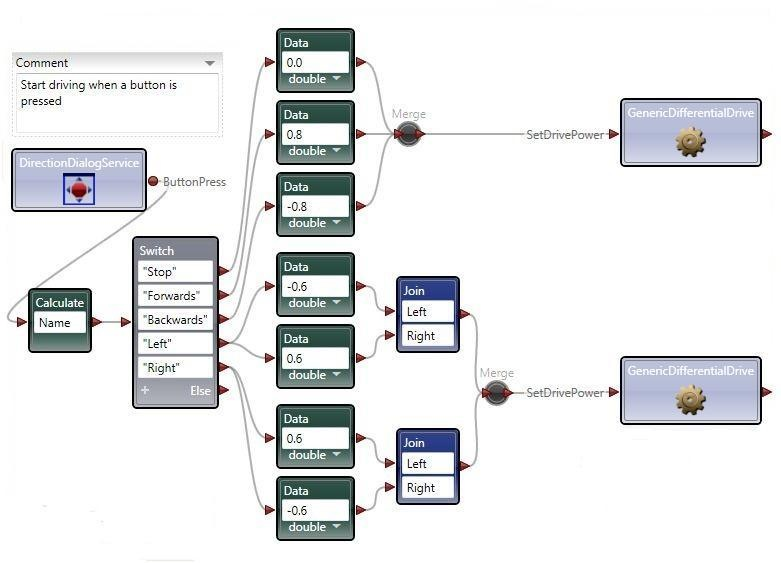
\includegraphics[scale=0.4]{rs.jpg}
\end{frame}

\begin{frame}
\frametitle{Визуальные(графовые) языки}
\framesubtitle{Получается на деле}
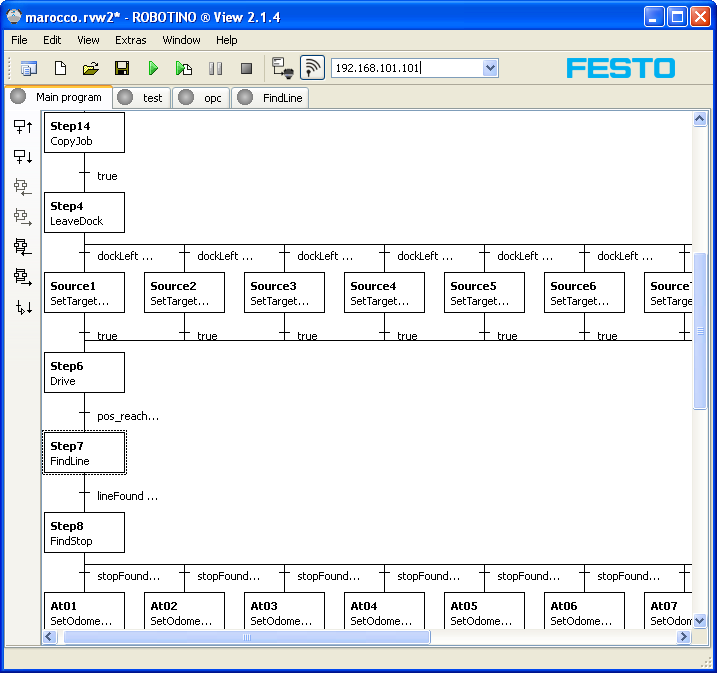
\includegraphics[scale=0.4]{robotino2.png}
\end{frame}


\section{Особенности программирования в мобильной робототехнике}
\begin{frame}
\frametitle{Технологии программирования}
\begin{itemize}
\item<1> Программируются готовые, выпускаемые серийно роботы и мехатронные
устройства
\item<2> \alert{Роботы разрабатываются самостоятельно и их компоненты меняются
во времени}
\item<1-> Язык программирования компонент - С,С++,Java, Python, C\#
компонент(модулей/агентов/сервисов).
\item<1-> Взаимодействие программных компонент через сети IP и RPC
(Remote Procedure Call, удаленный вызов процедур)
\end{itemize}
\end{frame}


\subsection{Недостатки традиционного подхода}
\begin{frame}
\frametitle{Недостатки традиционного подхода}
\begin{itemize}
  \item<1-> RPC подразумевает вызов уже существующих функций, в то время как
  процесс разработки сопровождается их созданием. Таким образом появляется
  необходимость постоянного обновления протокола и программ бортовой ЭВМ, а 
  обновление программ бортовой ЭВМ требует довольно длительной
  процедуры ``перезагрузки``  
  \item<1->Программы бортовой ЭВМ реализованы на компилируемом языке и
  любое обновление требует их повторной компиляции
  \item<1-> Традиционно используемые языки программирования неудобны для частой
  модернизации программ
\end{itemize}
\end{frame}

\section{Предлагаемый подход}
\begin{frame}
\frametitle{Предлагаемый подход}
\begin{itemize}
  \item<1>Перейти от использования компилируемого языка со статической
  типизацией к динамическому интерпретируемому языку
  \item<1>Обеспечить возможность изменять ПО бортовой ЭВМ без необходимости
  перезагрузки и, по-возможности, остановки.
  \item<1>Упростить процесс развертывания ПО на бортовой ЭВМ
  \item<1>Реализовать возможность распределения между бортовой ЭВМ и пультом
  управления не только модулей, но и отдельных строчек программного кода 
\end{itemize}
\end{frame}

\subsection{Интерпретируемый динамический язык}
\begin{frame}
\frametitle{Интерпретируемый динамический язык}
Использование в качестве основного языка программирования 
интерпретируемого динамического языка позволяет:
\begin{itemize}
  \item<1-> Устранить необходимость в файлах конфигурации.   
  \item<1-> Устранить этап компиляции для ПО бортовой ЭВМ
  \item<1-> Легко вносить незапланированные изменения в ПО бортовой ЭВМ в
  полевых условиях
\end{itemize}

\end{frame}

\subsection{Тьюринг-полный протокол}
\begin{frame}
\frametitle{Тьюринг-полный протокол}
\begin{itemize}
  \item<1> Изменение аппаратной составляющей робота или мехатронного устройства
  требует соответствующего изменения и программной составляющей. Как правило, за
  этим также следует изменение управляющего протокола (т.е. добавление новых
  команд или удаление существующих)
\item<1> Протокол управления это, фактически, язык программирования, и его можно
оценить с точки зрения полноты по Тьюрингу
\item<1> Вместо постоянного наращивания (вслед за аппаратной составляющей)
языка-протокола, имеет смысл сразу реализовать тьюринг-полный протокол.
\end{itemize}
\end{frame}

\subsection{Общее высокоуровневое адресное пространсво}
\begin{frame}
\frametitle{Тьюринг-полный протокол}
\framesubtitle{Общее высокоуровневое адресное пространсво}
Использование такого подхода и рефлексии языка позволяет получить доступ к общему
высокоуровневнему адресному пространсву, где проиходит адресация не отдельных
байт памяти, а высокоуровневых структур и, как слествие:
\begin{itemize}
	\item<1>Появляется возможность без дополнительных усилий получать
	телеметрические данные с одного робота на нескольких компьютерах 
	\item<1>Модифицировать отдельные участки программы непосредсвенно во время
	работы робота
	\item<1>Свободно перемещать участки программ между бортовой эвм и компьютером
	разработчика.
\end{itemize}
\end{frame}



\subsection{Язык Python}
\begin{frame}
\frametitle{Язык Python}
\framesubtitle{Почему Python, а не ruby/perl/tcl/lua/scala/\ldots}

\begin{itemize}
	\item<1>Простой и компактный синтаксис облегчает не только программирование, но
	и кодогенерацию
	\item<1>Простота интеграции с готовыми системами, созданными на С
	\item<1>Распространенность. Python используется более чем в 1400
	программах, входящих в комплект поставки Linux Ubuntu
	\item<1> Наличие открытых и эффективных сторонних библиотек: mathplotlib
	(графопостроитель), scipy (пакет математических библиотек) и др.,
	позволяющих почти полностью воспроизвести возможности mathlab в составе разрабатываемого ПО
\end{itemize}
\end{frame}

\begin{frame}
\begin{center}
\begin{LARGE}
Спасибо за внимание
\end{LARGE}
\end{center}
\end{frame}

\end{document}